\chapter{Literature review}

This chapter provides a systemic perspective on the labour 
markets supported by the literature. It starts with a brief 
discussion of the economic theory that governs labour markets, 
followed by an overview of different implementations of 
microsimulation models with an emphasis on the ILUTE framework. 
Finally, this chapter closes with a discussion of the gaps 
that guide the work in the subsequent chapters. Although the 
economic literature on this subject is extensive, this section 
is mainly based on the concepts and ideas stated by
\citep{Benjamin2021,Borjas2020,Kaufman2003,Smith2003}

\section{The economic theory of labour markets}

Labour markets are defined by the interaction of three principal agents\footnote{Unions can be analyzed as an additional agent depending on local legislation, and the union's influence power, among others \citep{Borjas2020}}: workers, firms, and governments, each with their subgroups, objectives, and agendas \citep{Benjamin2021}. On one side, workers are trying to sell their labour at the highest price, the \textit{supply side}, while on the other side, firms are trying to buy the labour at the lowest price, the \textit{demand side}. The regulations imposed by governments constrain these interactions between workers and firms. 

Different factors influence decisions made by individuals and companies and affect individual and group outcomes, such as earnings, type of employment, work hours and wages. Therefore, the primary objective of interactions within the labour market is to negotiate and agree on two key elements: wages and type of employment \citep{Benjamin2021}. 

The wage is the element that facilitates the exchange between agents in the labour market but also allocates labour to the most efficient use in terms of occupations, industries, and regions within a market economy. This allocation encourages productivity improvements, job search and mobility, and investments in human capital through training and education \citep{Benjamin2021}. For firms, especially in sectors heavily dependent on the labour force, such as agriculture or manufacturing, wages are crucial in determining the prices of goods and services \citep{Borjas2020}.

In a perfect competitive model, wages are only determined by the interactions of supply and demand, but the assumptions of this model are rarely met. A more realistic model assumes that individuals are heterogeneous and that there are differentials in the wage determination. In this scenario, wages are determined by the market interaction given the individual characteristics of the worker and the job offered \citep{Kaufman2003}. \citet{Smith1910} defines five principles that govern this differential in compensations: how pleasant or unpleasant is the job, how easy it is to learn the job, the stability of the job, the responsibility level, and the probability of success in that job. These principles are still applicable to most modern labour market configurations. 

On the other hand, individuals and firms negotiate the type of employment, which refers to the characteristics of the job, such as the number of hours, flexibility, long-term stability, benefits, and associated risks. From the worker's perspective, the desired employment type is related to their values and preferences. Some individuals will be willing to work longer hours to earn more, while others prefer a balance between work and life. From the firm's perspective, the type of employment depends on the industry, the level of production, and the decisions within specific economic cycles. If the demand for a good is high and the economy is growing, a company would increase its labour force, while if the demand for the good drops, the firm will be forced to reduce its workforce. 

Given the importance of wages and employment type in negotiation, the subsequent sections review these concepts for both sides of the market, focusing on the short- and long-term decisions.

\subsection{Labour supply}

Microeconomic theory states that the worker's behaviour can be explained using the neoclassical model of consumption-leisure choice. In this theoretical model, individuals exchange their leisure time for the consumption of goods —represented by the income received from working. The combination of leisure and consumption provides some level of satisfaction, measured as \textit{utility}, which is related to the values and preferences of each person. Hence, an individual entering the market aims to maximize their utility by choosing the best combination of leisure time and consumption. 

Time is scarce, so individuals make decisions under a constrained scenario in which short-term choices are limited to the available daily time after sleep. In contrast, long-term decisions are primarily defined in extended periods and involve a more thoughtful process. 

\subsubsection{Short-term decisions}

An individual's first and most important decision is whether to enter the labour market. According to \citet{Borjas2020}, every individual has a wage rate, known as \textit{reservation wage}, that motivates them to work. This wage rate reflects how much an individual values their leisure time but also includes some information about other sources of income such as investments or inheritances —also known as \textit{non-labour income}. 

A person who highly values their leisure time or has a non-labour income covering their basic expenses could have a higher reservation wage. In comparison, someone indifferent to leisure time or without another source of income could have a lower reservation wage. Therefore, the decision to participate or not in the labour market will be given by comparing the market and reservation wage rates. If the market wage exceeds the individual's reservation wage, this person will be motivated to work; otherwise, this person will remain out of the labour market. 

After deciding to participate in the labour market, individuals choose how many hours to work. This choice is modelled by constructing labour supply curves using the same consumption-leisure model. In this model, any increment in the market wage above the reservation wage leads to working more hours until the individual's choice between leisure and consumption is optimal. However, this model assumes that people only allocate their time to leisure or work. Still, there are different activities related to household production that are not considered under this model \citep{Borjas2020}. To overcome this issue, the \textit{household production function} allows the time allocation to be modelled based on the joint decision within the household unit. \citet{Benjamin2021} point out that this collective approach explains the recent changes in the Canadian workforce composition, in which more women are participating in the labour market, and the two-earner family groups are dominating the labour market structure.

In the household production function, the available time in a household is allocated based on the potential earnings of each individual, the dollar value of goods they want to consume, and the dollar value of the goods produced in the household\footnote{These goods are consumed at home and cannot be exchanged in any market. Some examples are childbearing, cooking, and cleaning.}. Some findings in historical data have demonstrated that optimal time allocation for a household is given mainly by the potential earnings of the individuals, in which the person with higher wages tends to work more hours while the other individuals will increase their participation in household activities \citep{Borjas2020}. However, introducing different technologies in recent years has changed this optimal allocation by improving the production of household goods and services \citep{Benjamin2021}. 

\subsubsection{Long-term decisions} 

The leisure-consumption model assumes that individuals make decisions only focused on the present by assessing the factors prevailing in one specific period. However, \citet{McCurdy1980} demonstrated that individuals make long-term decisions based on the expected wage changes during the life cycle. In this model, any wage change has two effects: an increase or decrease in the hours dedicated to work.

In the first case, the \textit{substitution effect}, any wage increase makes leisure time more expensive and motivates individuals to work longer. This effect is usually observed in people starting or at the mid-point of their professional careers. In the second case, the \textit{income effect}, any increase in the non-labour income produces a rise in the utility level, giving the individuals the opportunity to work fewer hours. This effect is commonly observed among experienced individuals or people close to retirement. Besides the decisions based on the worker's life cycle, individuals also adjust their labour supply based on business cycles. According to \citet{Borjas2020}, during recession periods, some household members who are out of the labour force (\textit{secondary workers}) can be motivated to enter the labour market if the \textit{primary worker} loses their job. 

Besides wages and earnings, some long-term decisions individuals make during their life cycle influence their choices related to work, such as childbearing, education, and retirement. These events might not be relevant to all individuals in the labour market but are closely related to individual preferences and the socioeconomic context. For childbearing, according to \citet{Angrist1998}, maternity reduces female labour supply with a lower effect among college-educated women or households where the male receives high wages. In contrast, they found minimal changes in the male labour supply in response to the birth of a child. They conclude that the decision to increase the family size is absorbed by the reduction of women's earnings or by purchasing child-care services, and the collateral effects are perceived both in the short and the long term based on the household income. 

In the case of education, the human capital theory explains how individuals perceive the potential benefits of acquiring additional skills by forgoing current income in a similar approach to assessing an investment. \citet{Benjamin2021} argue that the motivation to enroll in a program is related to the wages the market is willing to pay. Under this perspective, firms are also eager to pay higher salaries and hire highly educated workers based on the assumption that these individuals will be more productive. However, the “ability at work” is not only obtained through education but can also be acquired through on-the-job training. This evidence suggests that both education level and experience can predict wages in the labour market. 

Finally, the decision to retire is based on a combination of different factors such as wealth, earnings, and the balance in the pension accounts. As described by \citet{Benjamin2021}, the main factor is the wealth and earnings of the individual, in which the non-labour income plays a crucial role in determining the retirement age. They also find that other factors such as health conditions, the family and the nature of work can influence the decision based on the individual attributes. Some health conditions can motivate early retirement, especially in those sectors that demand physical activity from their workers —\textit{blue-collar} jobs, while in other physically demanding jobs, retirement can be postponed —\textit{white-collar} jobs. Also, changes in family composition and size in recent years could motivate people to remain longer in the labour market \citep{Baker1999}.

\subsection{Labour demand}

On the demand side of the labour market, firms are the agents that use labour to produce goods and services. In product markets, labour is considered a \textit{derived demand} because it is one of the production factors. The relationship with product markets makes labour demand dependent on the prices of goods and services and the structure of these markets. That means that the decisions of firms operating in a competitive market will differ from those in a non-competitive market (such as monopsony or oligopoly). However, when firms enter the labour market, they aim to maximize profits and minimize costs regardless of the market structure \citep{Benjamin2021}. 

Like the labour supply, firms' decisions vary between short- and long-term in relation to the main factors in the firm's production function: labour, capital, and technology \citep{Borjas2020}. In the short term, it is assumed that capital and technology remain fixed, and labour is the only factor firms can use to modify their production. While in the long term, all factors can vary. 

\subsubsection{Short-term decisions} 

As profit maximizers, firms will adjust their factors to achieve the lowest cost of production. While changes in some factors can take more time to be implemented —the construction of a new plant or the preparation for an IPO to raise equity capital from investors, labour is the only factor that can be easily modified in the short term. Under this scenario, firms will adjust their labour demand based on the cost of labour (wages), their worker's productivity, the firm's production level, and the prices in the product market \citep{Kaufman2003}. 

The \textit{marginal productivity theory} evaluates these factors to model the firm's demand for labour under the assumption that the firm operates in a perfect competition market. Hence, a firm will increase its workforce by one worker if the productivity increment given by this additional worker is higher than the cost of hiring it —represented by the wage \citep{Kaufman2003,Borjas2020}. Given that the amount of capital is fixed, there is no substitution effect, and the labour demand will experience a diminishing marginal productivity and scale effect \citep{Benjamin2021}. That means there is an optimal point at which the number of workers maximizes the firm's profits, and after or before that point, the firm is in a non-optimal scenario. This optimal number of workers will be the firm's short-term labour demand. 

However, quantifying the worker's productivity is not an easy task. \citet{Kaufman2003} state that the difficulty of measuring individual productivity increases with the firm size, as more extensive production lines involve many workers in the production process. 

\subsubsection{Long-term decisions} 

As all factors can vary in the long run, labour can be substituted for other inputs such as capital. This substitution is based on the relative prices of both labour and capital. Therefore, the long-term decision to increase or decrease the labour force is subject to wages and the economic outlook that defines the cost of capital \citep{Kaufman2003}. Under a scenario where wage rates are increased, if the output remains the same, it will impact the quantity of labour demand because firms will use more capital instead of labour —a \textit{substitution effect}. Likewise, if the amount of the output is reduced, the firm will further reduce their labour demand because it will be in a suboptimal scenario —\textit{scale effect}. 

Technology also plays a key role in the long-term demand for labour. As technological breakthroughs increase productivity and efficiency, it also increases the demand for labour—scale effect. However, some occupations are replaced by innovations, making some skills obsolete —substitution effect. 

\subsection{Market interaction}

Labour markets have unique characteristics that differ in structure from other product markets. \citet{Kaufman2003} identifies some key differences, such as the item exchanged (labour) is embodied in the human being, the long-term nature of employment relationship, the heterogeneity of workers and jobs, and the diversity of markets. These differences impact the agents' decision-making process, the labour market interactions, and the market equilibrium. 

In a perfect competitive single-market model, the equilibrium is reached when workers and firms agree upon the market wage rate. This market-clearing state assumes that all individuals and firms meet their objectives\footnote{All individuals eager to work at the market wage are employed, and all firms eager to pay the market wage hire the labour force they required. }. However, under an equilibrium state, the difference between what the firms are willing to pay and the wage rate is known as producer surplus. Likewise, the difference between what workers are willing to earn and the wage rate is known as worker surplus. The aggregate of producer and worker surplus are the economic gains for participating in the trade or entering the market —also known as \textit{gains from trade} \citep{Borjas2020}. 

Under this equilibrium state, the efficient allocation of workers to firms is the one that maximizes the gains of trade. As wages are the mechanism to allocate resources in the labour market, wages could be the primary driver of occupation choices and labour mobility between different markets, risk environments, and regions \citep{Borjas2020}. However, a static market equilibrium may be more a theoretical concept than a state reachable in the real world. According to \citet{Borjas2020}, many labour markets do not adjust so quickly to supply and demand shocks. He illustrates this concept using the market for new engineering graduates as an example, in which the market fluctuates between periods of excess demand for labour and periods of excess supply. 

This fluctuation generates a cyclical trend in the entry wages for engineering graduates —also known as the \textit{Cobweb model}. In a period of excess demand for engineers, entry wages tend to be higher as a reflection of the market interaction. Thus, a new generation of students enroll in engineering programs using the current information from the market. Nevertheless, this information failure could create a future excess of supply once the new generation graduates from engineering school and enters the labour market. Therefore, the idea that equilibrium is more oscillatory than static helps to represent many other markets characterized by systematic booms and busts \citep{Benjamin2021,Borjas2020}. 

\subsection{Job search and worker-job matching process} 

In the perfect competition model, firms and workers have all the information to enter the market. However, the information flow is asymmetrical because neither workers nor firms are fully informed when entering the market. This information asymmetry implies that agents invest time gathering information about the labour market before a match \citep{Borjas2020}. 

During the search phase, workers can choose from a set of potential offers, each with some differences in the wage, while firms can choose from a set of applicants, each with some differentials in their skills and experiences. According to \citet{Benjamin2021}, these differentials can be represented by the \textit{wage offer distribution}, which reflects the probability distribution of the wage offers received by an individual. Although this distribution is limited to the job opportunities available to that individual at that time, it is a proxy measure that reflects the market value of the worker. 

In the job-matching phase, the individual sets their \textit{reservation wage} —sometimes called \textit{asking wage}— and sequentially assesses different opportunities, comparing them with the reservation wage, until they reach one above their expectation. Although the individual can wait to meet their expectations, there is an opportunity cost for not taking an offer below the reservation wage. This opportunity cost adjusts the reservation wage based on their individual preferences. Some individuals will have enough patience and savings to wait for the expected offer, while others will adjust quickly their reservation wage to match the wage offer distribution \citep{Benjamin2021,Borjas2020}. Nevertheless, the adjustment of the reservation wage can also be performed by comparing it with the current market value distribution —represented by the wage offer distribution. If the reservation wage is outside the distribution, the individuals will adjust their expectations accordingly to increase the likelihood of being hired. 

\subsection{Wage definition}\label{section:wage_definition} 

On the demand side, salaries can be defined by a \textit{Hedonic model} that explains the wage based on the worker's perceived job risk \citep{Borjas2020}. Hence, riskier jobs have higher wages to incentivize people to accept them. However, the hedonic model can be extended beyond the definition of job risk by including other job attributes such as skill level, location, amenities, and long-term stability. \Cref{eq:1} presents the general form of this model in which $w_i$ is the wage of worker $i$, $\rho_i$ is the probability of injury, $\beta_j$ is the parameter for the $j^{th}$ job characteristic, and $V_{ij}$ is the $j^{th}$ job characteristic of the worker \citep{Borjas2020}.

\begin{equation}\label{eq:1}
w_i=\alpha+\sum_{j=1}^{J}\beta_jV_{ij}+\rho_i
\end{equation}

On the supply side, human capital theory and life-cycle labour supply models have also used linear models to estimate wages as a function of several individual attributes. In human capital theory, wages reflect the accumulation of capital such as education and job experience, while in the life-cycle labour supply approach, wages are defined by some individual attributes relative to each industry, also known as \textit{fixed factors} \citep{Borjas2020,Sullivan2010}. 

\section{Practical approaches for modelling labour markets} 

This section explores some implementations of labour market microsimulation models that manage earnings, transitions, and events as endogenous components. As the work of this thesis is expected to be used within the transportation and urban planning setting, the first part reviews the urban microsimulation framework ILUTE\footnote{To the author's best knowledge, most of the land use-transportation interaction models treat labour markets and employment exogenously, and ILUTE is one of the first to include it as an endogenous component. \citet{Harmon2013} presented a comprehensive literature review about the approaches to include labour market on different land use-transportation models but most of them are focused on just one side of the labour market, the demand or supply. By the time this thesis is written, most of these findings remain the same.}. The second part presents an overview of some microsimulation frameworks used for modelling labour markets in other contexts, such as demographic analysis and pension policy testing, to compare other approaches outside the transportation context.

\subsection{ILUTE framework}\label{section:ilute}

The Integrated Land-Use, Transportation, and Environment framework (ILUTE) is an urban microsimulation model that simulates the activities of individual agents as they evolve in a specified period. This framework has been tested using data from the Greater Toronto Area \citep{Salvini2005}. In this modelling system, census population data are synthesized to produce agents that represent the population of the GTA and simulate different high-level decisions (residential location, firm location, auto ownership) and low-level decisions (activity scheduling, trip mode selection). The interactions between different agents are represented as market transactions, and the outcomes are the inputs to other sub-markets. 

The ILUTE implementation consists of different sub-models that simulate interactions or processes in urban areas, as shown in \Cref{fig:ilute}, in which the labour market was a sub-model “Under development” by the time that document was released.

\begin{figure}[h]
    \centering
    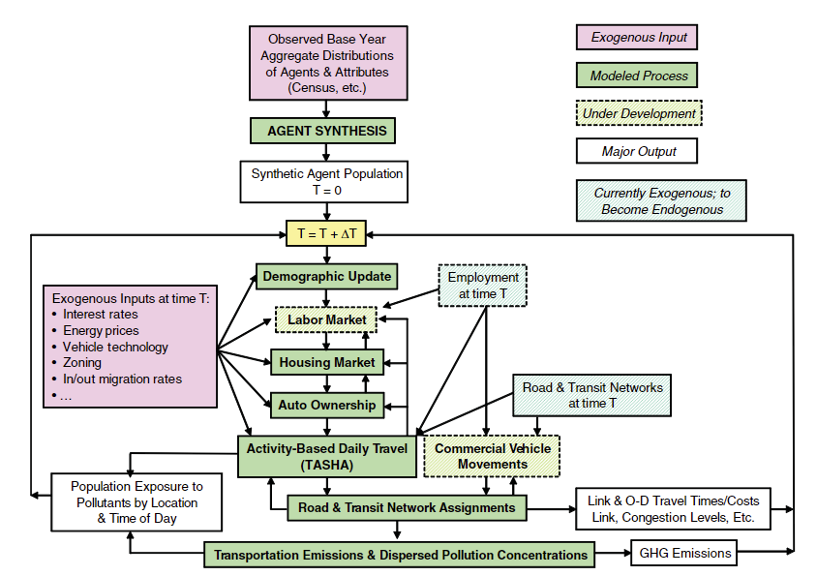
\includegraphics[width=0.8\textwidth]{images/ch2_ilute/ilute.png}
    \caption{Flowchart of ILUTE processes \citep{Miller2021}}
    \label{fig:ilute}
\end{figure}

Posterior works of \citet{Hain2010} and \citet{Harmon2013} proposed a procedure to simulate labour markets within the ILUTE framework. \citet{Hain2010} prepared a series of linear regression models to predict wages based on some attributes and characteristics of the worker. In this work, he explores different predictors of wages, distinguishing between full-time, part-time, annual, and hourly salaries following the hedonic econometric approach reviewed in \Cref{section:wage_definition}. The same approach was used to estimate the hours of work based on the attributes of the worker, but the linear regression models were not statistically significant.

In addition, Hain estimated a transition model using three binary logit models that calculate the probability of a person transitioning between being employed to unemployed, unemployed to out of the labour force, and out of the labour force to unemployed. Hain recognized the need for a fully endogenous microsimulation model of the labour market that treats both the demand and supply sides as agents. 

Based on Hain's work, \citet{Harmon2013} built an agent-based model using the wage and transition models. He proposed a simplified firmographic model representing the endogenous creation and deletion of jobs in the labour market. He also used a series of linear regression models based on GDP and unemployment rate to predict each period's added or deleted jobs per sector. Moreover, he estimated a series of cumulative distribution functions to assign different attributes to the worker and job class, such as industry, occupation, job type (full or part-time), firm size, and location. 

Using these models, Harmon proposed a job-matching algorithm in which a random pool of candidates is evaluated, and the worker with higher utility accepts the offer \citep{HarmonMiller2018,HarmonMiller2020}. This job-search and matching process is summarized in \Cref{fig:job_matching}. All models are updated for each timestep (defined in ILUTE as a year), simulating the labour market's long-term dynamic as agents and economic conditions evolve over time.

\begin{figure}[h]
    \centering
    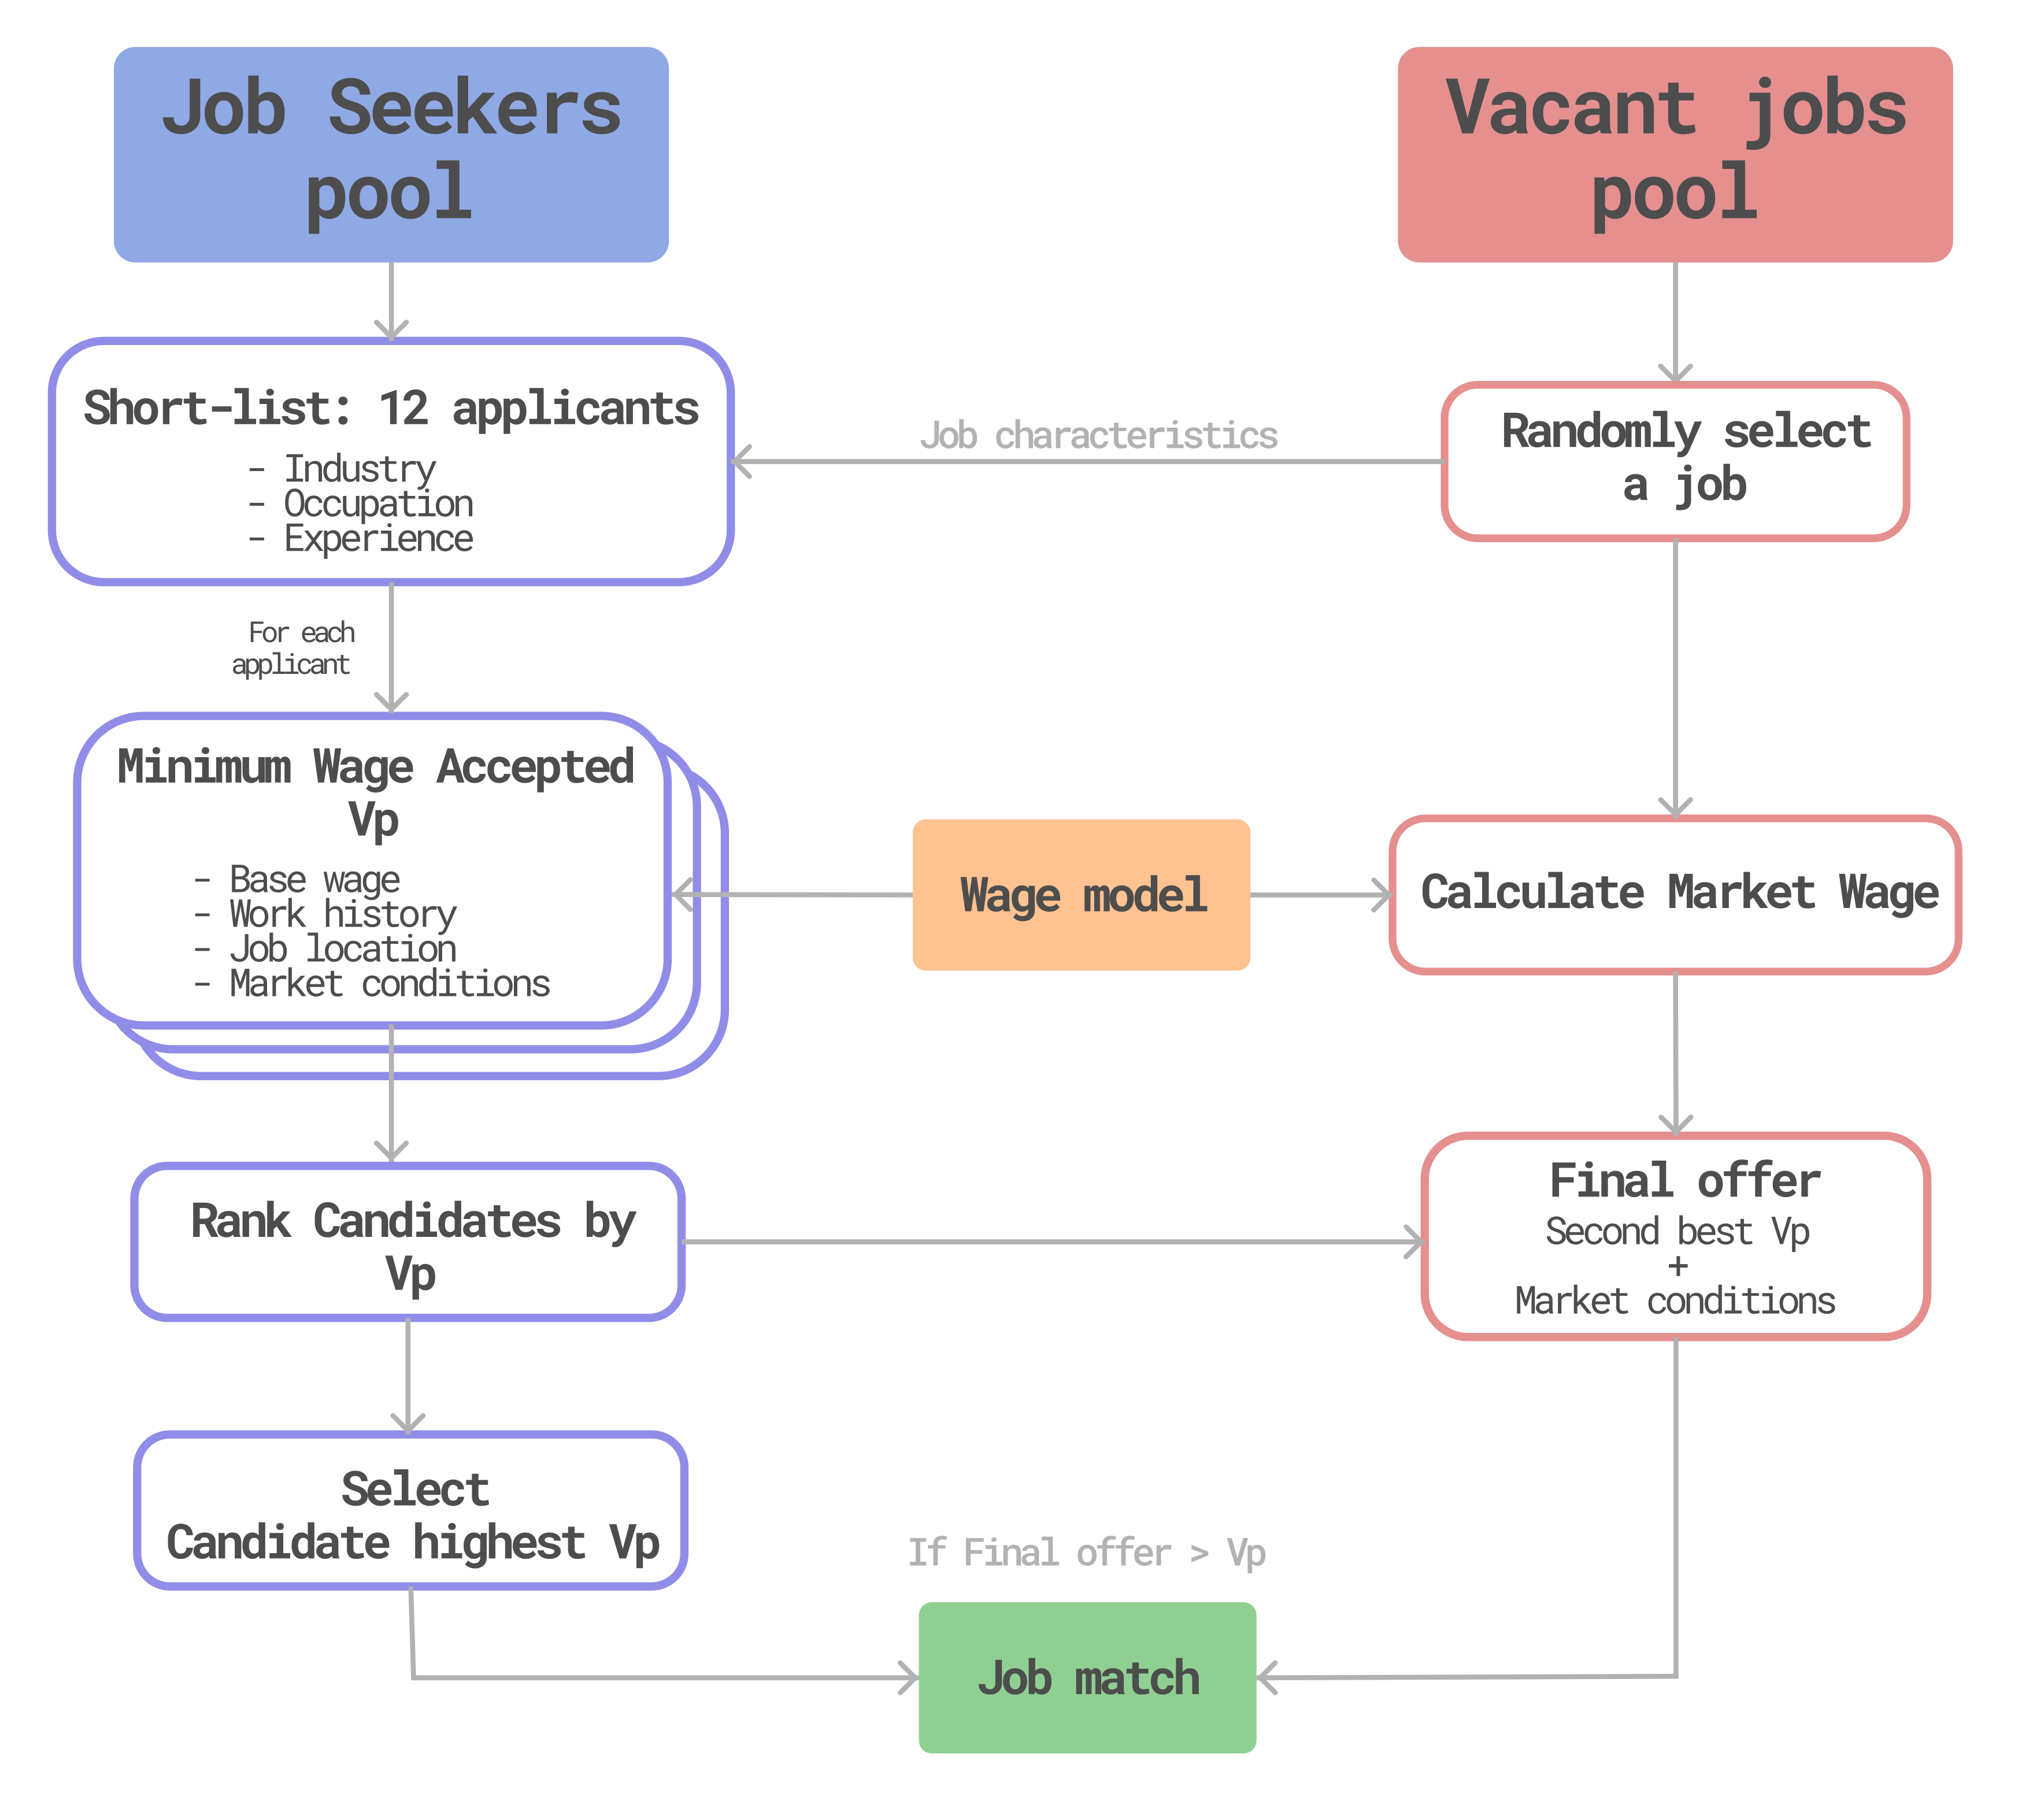
\includegraphics[width=0.8\textwidth]{images/ch2_job_matching/job_matching.png}
    \caption{Job search and matching process in ILUTE (Adapted from \citet{Harmon2013})}
    \label{fig:job_matching}
\end{figure}

The simulation results have been compared with actual data from 1987 to 2006, demonstrating an accurate estimation of employment counts by industry and occupation. However, as \citet{Harmon2013} pointed out, more research is needed to fully represent the internal interactions in the labour market. Both Hain and Harmon propose that this should be accomplished by generating a fully endogenous firmographic model that simulates the birth and death of firms while providing the evolution of jobs (creation and deletion) during these business cycles. 

Moreover, according to \citet{Harmon2013}, the wage model underestimates wages in relation to prior experience and tenure levels, directly impacting the matching algorithm's long-term stability. As the models were estimated using single-year datasets, Harmon points out the need to validate the temporal stability of the parameters for the job demand and supply models. 

\subsection{Other dynamic microsimulation frameworks} 

The following models are examples outside the transportation planning setting that use a microsimulation approach to assess the long-term impact of policy changes in the pension and fiscal systems. Although some models are being updated or replaced by new versions, this review provides evidence about the possible challenges and opportunities of implementing these microsimulation systems. 

\subsubsection{DYNACAN and Lifepaths (Canada) }

Statistics Canada has a long history of experimenting with dynamic microsimulation models to estimate and project some sociodemographic characteristics relevant to Canadian society, such as aging, pension plans, and health. This effort has produced several models, from DYNACAN in the early 1990s to the LifePaths in the early 2010s. DYNACAN and LifePaths are discontinued because Statistics Canada is developing a new dynamic socio-economic microsimulation tool\footnote{ This information was retrieved from: \url{https://www.statcan.gc.ca/en/microsimulation/index}, in February 2023}. 

The DYNACAN model is a dynamic microsimulation model used to estimate the impacts of policy changes in demographics, earnings and other characteristics related to the Canadian Pension Plan -CPP \citep{StatsCAN2018}. For the base year, DYNACAN uses over 212,000 agents representing a sample of the Canadian population for the 1971 census (starting database). The model consists of three modules: Part A assembles and prepares the data into a single hierarchical database for the following modules, Part B simulates the demographic events and employment earnings over time, and \\ Part C calculates the CPP contributions and benefits for each agent. 

Regarding the labour market, DYNACAN models several events directly related to individuals' participation in the labour force. The events and the explanatory variables are summarized in \Cref{table:dynacan}. 

\renewcommand{\arraystretch}{1.5}
\begin{table}[!h]
    \begin{tabular}{p{4cm}p{10cm}}
        \textbf{Event} & \textbf{Explanatory Variables} \\
        \hline
        \rowcolor{lightgray} Education & Gender, age, parents' education, living arrangements, house-ownership status, marital status, children \\

        Employment status (worked less/more than 48 weeks) & Gender, age, marital status, children, disability status, retirement status, and working status in previous years \\

        \rowcolor{lightgray} Female exclusion from the labour force & Age (>21), gender (female), marital status, children, labour force participation in previous years\\

        Annual weeks worked (0, 1-47, 48 or more) & Age, gender, marital status, tenure in current job, education level, children, children's age, unemployment rate\\ 

        \rowcolor{lightgray} Weakly wage & Age, gender, marital status, children, education level, unemployment rate, previous year earnings, employment status, tenure in current job \\

        Income from employment & Product of wage time weeks worked\\

        \rowcolor{lightgray} Retirement age & Age, disability status, gender, CPP contributions\\
        \hline
    \end{tabular}
    \caption{\label{table:dynacan} Labour market-related events on DYNAMO (Adaptation from \citet{Joseph1997}}
\end{table}


Although there is no official documentation about the procedures in this model, most of the events combine rule-based models and linear or logistic regressions that capture the agent's behaviour \citep{Joseph1997}​. All simulations are performed using the Monte Carlo technique. Since the model is not a market-clearing model, there is no interaction between firms and workers and no feedback from the pension system provision, labour market, savings or demographic modules \citep{Joseph1997}.

DYNACAN was replaced by LifePaths, which was intended to be a multipurpose microsimulation model that simulates a large sample of individuals in much more detail than the DYNACAN. LifePaths uses a variety of Canadian microdata, which makes it suitable for analyzing government policies of a longitudinal nature. It supports different dimensional analyses such as cross-sectional, over individual lives, between cohorts and over generations \citep{StatsCAN2013}. LifePaths simulate different life events through probabilistic functions, and events are modelled as random processes in which the occurrence of an event is conditional to the previous history plus a stochastic component. 

Similarly to DYNACAN, LifePaths simulates different labour market-related events based on the sociodemographic characteristics of each agent. \Cref{table:lifepaths} summarizes these events and their explanatory variables.

\renewcommand{\arraystretch}{1.5}
\begin{table}[!h]
    \begin{tabular}{p{4cm}p{10cm}}
        \textbf{Event} & \textbf{Explanatory Variables} \\
        \hline
        \rowcolor{lightgray} Student Employment & Gender, province of residence, status in the parental home, variables representing seasonal patterns \\

        Employment status & Gender, age, province of residence, education level, children, marital status, spouse's employment status \\

        \rowcolor{lightgray} Retirement \newline (if age>60) & Age, gender, province of residence, family characteristics, and education level. \\ 

        Hours worked per week & Age, gender, education level, province of residence, family characteristics, student status, job tenure\\

        \rowcolor{lightgray} Maternity leave & Age, marital status, education level, employment status, tenure in current job \\

        Weekly earnings & Age, gender, education level, field of study, province of residence, and immigration status \\
        \hline
    \end{tabular}
    \caption{\label{table:lifepaths} Labour market-related events on LifePaths Adaptation from \citep{StatsCAN2013}.}
\end{table}







Lifepath's official documentation does not provide detailed information about the procedures and models. It only states that the behavioural component combines rule-based models with logistic and linear regressions. 

\subsubsection{APPSIM (Australia)} 

The Australian Population and Policy Simulation Model (APPSIM) is a microsimulation model developed by the National Centre for Social and Economic Modelling at the University of Canberra to evaluate the impact of future social and fiscal policies until 2050. According to \citet{Keegan2007} APPSIM uses a 1\% sample of the 2001 census as the initial population. The primary individual characteristics are obtained from the census, but other microdata sources are used to impute additional characteristics such as earnings and employment history. Using a series of multinomial logit models, the model uses these data sources to estimate the transition probabilities for different states. The model updates the agent's states annually using Monte Carlo simulation. 

APPSIM is structured as a modular framework in which agent states are updated annually. The modelled states range from demographic events such as births, leaving parents' home, marriage, and education to more specific ones such as the states in the labour market or health conditions. Regarding the labour market module, APPSIM classifies states in labour force status, employment dedication, and employment type. One essential process in APPSIM is the “Alignment” of simulation results with historical data. This process ensures that the microsimulation is aligned with aggregated results in macro projections and that the model results are stable in the long term. 

\subsubsection{ELSI (Finland)} 

The ELSI framework is a microsimulation model created by the Finnish Centre of Pensions to analyze employment trajectories in the context of the pension system. This model is an individual-level simulation alternative to the semi-aggregated model (LTP) used by the Finland Ministry of Finance. One of the advantages of ELSI is the ability to model immediate and long-term effects of policy reforms related to the labour market and pension system \citep{Tika2020}. 

ELSI uses a different approach than DYNACAN, LifePaths, and APPSIM because the transition probabilities are not obtained using behavioural equations (logistic regressions or multinomial logit models). Instead, ELSI calculates the transition between states using probability functions following a random Markov process in which the future state only depends on the current state. 

For the labour market model, ELSI defines 21 states in six categories: employed, unemployed, outside the labour force, sick, retired, and deceased. Given that the purpose of this model is to evaluate pension-related policies, the granularity of states is related to the relationship with the pension system in that state. 

One key component of the ELSI model is that the earnings model calculates the labour and pension-related earnings separately, which generates a feedback loop with the labour market transition module. This representation introduces the effect of non-labour income in the transition decisions in the labour market. The annual salary is estimated using a hedonic regression based on some individual's characteristics and adds a random component to simulate the variability of wages between similar individuals. \citet{Tika2020} use an asymmetric Laplace distribution for modelling this random component. 

\section{Conclusions of the literature review and current gaps} 

The literature review presented in this chapter provides evidence that labour markets possess structural differences from other markets in the economy because the product, labour, is attached to individuals. This attachment increases the complexity of individual decisions in the short and long term because the possible outcomes can significantly impact other parts of life. Moreover, much of the information the agents share in labour markets is incomplete or asymmetrical, affecting market efficiency and producing sub-optimal equilibrium. 

In this context, microeconomic theory is helpful to explain the rationality behind decisions in the labour market. However, the assumptions of these models do not fit with most of the actual conditions of labour markets. The field of econometrics uses observed data to evidence the theoretical structure of labour markets in an aggregated or semi-aggregated way. However, these models can be extended into a microsimulation approach that captures the heterogeneity of the agents and better represents the interaction between firms and workers. 

Although most examples of microsimulation models in the labour market have been developed with a unique purpose, a new generation of dynamic models is developed with a multipurpose perspective. ILUTE follows this idea by modelling different systems within the urban context with the idea that the world operates as a system of systems. 

The results obtained by Harmon using the Agent-Based implementation of the Labour Market module in ILUTE demonstrate that the microsimulation approach is a good representation of the market at an aggregate and semi-aggregated level. However, additional efforts should be focused on improving the models that govern the behavioural decisions within the module. 

In particular, Harmon points out that the existent wage model underestimates salaries when comparing the intercepts of the full-time with the part-time models. One possible explanation for this issue is the quality of the values of worked hours reported in SLID. As this survey was performed once every year, respondents could not recall this number correctly. Therefore, a possible approach is to use annual salary instead of hourly wage. This variable, also reported in SLID, could be more reliable and produce better results. 

Moreover, the deterministic nature of Hain's model could be an additional source of the log-run instability of the model. As the linear model represents the average salary for an individual with specific attributes, all individuals sharing those attributes will have the same predicted salary. From the simulation perspective, this approach is missing an essential component of reality, in which randomness can explain some differences in wages between individuals. Therefore, a model that includes this random component could improve the stability and behavioural representation of the agent-based model. 

This deterministic outcome could also affect the current implementation of the job-matching process. The current price-taker approach in which workers accept or decline a job offer does not consider that they assess the market by applying to different job offers and select the most optimal. Although Harmon's model adjusts the \textit{MinimumWageAccepted} by location and number of attempts, the wage model produces the same point estimate for all individuals with the same attributes, which translates into all job offers in one specific bucket being equally perceived by the workers. In reality, the wage differentials between offers make some more appealing than others, and the trade-off between the benefits and costs\footnote{Such as transportation and travel time costs} of each option is the decisive factor. Hence, including the random component in the salary representation in the ABM module could improve the job-matching process. 

Given these challenges and the importance of wages in the interaction between workers and firms in the labour market, this thesis proposes an alternative salary model that implements the missing random component and introduces some changes in the current structure of the Agent-Based model to represent the job-searching and matching process better. The proposed model uses the Bayesian inference approach to model the uncertainty in the prediction and produce probability distributions instead of point estimates. The details of this approach are covered in the following chapters. 